%  LaTeX support: latex@mdpi.com
%  For support, please attach all files needed for compiling as well as the log file, and specify your operating system, LaTeX version, and LaTeX editor.

%=================================================================
% pandoc conditionals added to preserve backwards compatibility with previous versions of rticles

\documentclass[notspecified,article,submit,moreauthors,pdftex]{Definitions/mdpi}


%% Some pieces required from the pandoc template
\setlist[itemize]{leftmargin=*,labelsep=5.8mm}
\setlist[enumerate]{leftmargin=*,labelsep=4.9mm}


%--------------------
% Class Options:
%--------------------

%---------
% article
%---------
% The default type of manuscript is "article", but can be replaced by:
% abstract, addendum, article, book, bookreview, briefreport, casereport, comment, commentary, communication, conferenceproceedings, correction, conferencereport, entry, expressionofconcern, extendedabstract, datadescriptor, editorial, essay, erratum, hypothesis, interestingimage, obituary, opinion, projectreport, reply, retraction, review, perspective, protocol, shortnote, studyprotocol, systematicreview, supfile, technicalnote, viewpoint, guidelines, registeredreport, tutorial
% supfile = supplementary materials

%----------
% submit
%----------
% The class option "submit" will be changed to "accept" by the Editorial Office when the paper is accepted. This will only make changes to the frontpage (e.g., the logo of the journal will get visible), the headings, and the copyright information. Also, line numbering will be removed. Journal info and pagination for accepted papers will also be assigned by the Editorial Office.

%------------------
% moreauthors
%------------------
% If there is only one author the class option oneauthor should be used. Otherwise use the class option moreauthors.

%---------
% pdftex
%---------
% The option pdftex is for use with pdfLaTeX. Remove "pdftex" for (1) compiling with LaTeX & dvi2pdf (if eps figures are used) or for (2) compiling with XeLaTeX.

%=================================================================
% MDPI internal commands - do not modify
\firstpage{1}
\makeatletter
\setcounter{page}{\@firstpage}
\makeatother
\pubvolume{1}
\issuenum{1}
\articlenumber{0}
\pubyear{2023}
\copyrightyear{2023}
%\externaleditor{Academic Editor: Firstname Lastname}
\datereceived{ }
\daterevised{ } % Comment out if no revised date
\dateaccepted{ }
\datepublished{ }
%\datecorrected{} % For corrected papers: "Corrected: XXX" date in the original paper.
%\dateretracted{} % For corrected papers: "Retracted: XXX" date in the original paper.
\hreflink{https://doi.org/} % If needed use \linebreak
%\doinum{}
%\pdfoutput=1 % Uncommented for upload to arXiv.org

%=================================================================
% Add packages and commands here. The following packages are loaded in our class file: fontenc, inputenc, calc, indentfirst, fancyhdr, graphicx, epstopdf, lastpage, ifthen, float, amsmath, amssymb, lineno, setspace, enumitem, mathpazo, booktabs, titlesec, etoolbox, tabto, xcolor, colortbl, soul, multirow, microtype, tikz, totcount, changepage, attrib, upgreek, array, tabularx, pbox, ragged2e, tocloft, marginnote, marginfix, enotez, amsthm, natbib, hyperref, cleveref, scrextend, url, geometry, newfloat, caption, draftwatermark, seqsplit
% cleveref: load \crefname definitions after \begin{document}

%=================================================================
% Please use the following mathematics environments: Theorem, Lemma, Corollary, Proposition, Characterization, Property, Problem, Example, ExamplesandDefinitions, Hypothesis, Remark, Definition, Notation, Assumption
%% For proofs, please use the proof environment (the amsthm package is loaded by the MDPI class).

%=================================================================
% Full title of the paper (Capitalized)
\Title{Análisis del mercado laboral en España}

% MDPI internal command: Title for citation in the left column
\TitleCitation{Análisis del mercado laboral en España}

% Author Orchid ID: enter ID or remove command
%\newcommand{\orcidauthorA}{0000-0000-0000-000X} % Add \orcidA{} behind the author's name
%\newcommand{\orcidauthorB}{0000-0000-0000-000X} % Add \orcidB{} behind the author's name


% Authors, for the paper (add full first names)
\Author{Catret Ruber, Pablo$^{1}$, Palazón Caballero, José
Miguel$^{1,*}$, Rosique Martínez, Marcos$^{1}$}


%\longauthorlist{yes}


% MDPI internal command: Authors, for metadata in PDF
\AuthorNames{Catret Ruber, Pablo, Palazón Caballero, José
Miguel, Rosique Martínez, Marcos}

% MDPI internal command: Authors, for citation in the left column
%\AuthorCitation{Lastname, F.; Lastname, F.; Lastname, F.}
% If this is a Chicago style journal: Lastname, Firstname, Firstname Lastname, and Firstname Lastname.
\AuthorCitation{Catret Ruber, P.; Palazón Caballero, J.M.; Rosique
Martínez, M.}

% Affiliations / Addresses (Add [1] after \address if there is only one affiliation.)
\address{%
$^{1}$ \quad Universitat de València - Escola Tècnica Superior
d'Enginyeria (ETSE) Avinguda de l'Universitat, 46100 Burjassot,
Valencia; \\
}

% Contact information of the corresponding author
\corres{Correspondence: \href{mailto:jomipaca@alumni.uv.es}{\nolinkurl{jomipaca@alumni.uv.es}}.}

% Current address and/or shared authorship








% The commands \thirdnote{} till \eighthnote{} are available for further notes

% Simple summary
\simplesumm{A Simple summary goes here.}

%\conference{} % An extended version of a conference paper

% Abstract (Do not insert blank lines, i.e. \\)
\abstract{A single paragraph of about 200 words maximum. For research
articles, abstracts should give a pertinent overview of the work. We
strongly encourage authors to use the following style of structured
abstracts, but without headings: 1) Background: Place the question
addressed in a broad context and highlight the purpose of the study; 2)
Methods: Describe briefly the main methods or treatments applied; 3)
Results: Summarize the article's main findings; and 4) Conclusion:
Indicate the main conclusions or interpretations. The abstract should be
an objective representation of the article, it must not contain results
which are not presented and substantiated in the main text and should
not exaggerate the main conclusions.}


% Keywords
\keyword{keyword 1; keyword 2; keyword 3 (list three to ten pertinent
keywords specific to the article, yet reasonably common within the
subject discipline.).}

% The fields PACS, MSC, and JEL may be left empty or commented out if not applicable
%\PACS{J0101}
%\MSC{}
%\JEL{}

%%%%%%%%%%%%%%%%%%%%%%%%%%%%%%%%%%%%%%%%%%
% Only for the journal Diversity
%\LSID{\url{http://}}

%%%%%%%%%%%%%%%%%%%%%%%%%%%%%%%%%%%%%%%%%%
% Only for the journal Applied Sciences

%%%%%%%%%%%%%%%%%%%%%%%%%%%%%%%%%%%%%%%%%%

%%%%%%%%%%%%%%%%%%%%%%%%%%%%%%%%%%%%%%%%%%
% Only for the journal Data



%%%%%%%%%%%%%%%%%%%%%%%%%%%%%%%%%%%%%%%%%%
% Only for the journal Toxins


%%%%%%%%%%%%%%%%%%%%%%%%%%%%%%%%%%%%%%%%%%
% Only for the journal Encyclopedia


%%%%%%%%%%%%%%%%%%%%%%%%%%%%%%%%%%%%%%%%%%
% Only for the journal Advances in Respiratory Medicine
%\addhighlights{yes}
%\renewcommand{\addhighlights}{%

%\noindent This is an obligatory section in “Advances in Respiratory Medicine”, whose goal is to increase the discoverability and readability of the article via search engines and other scholars. Highlights should not be a copy of the abstract, but a simple text allowing the reader to quickly and simplified find out what the article is about and what can be cited from it. Each of these parts should be devoted up to 2~bullet points.\vspace{3pt}\\
%\textbf{What are the main findings?}
% \begin{itemize}[labelsep=2.5mm,topsep=-3pt]
% \item First bullet.
% \item Second bullet.
% \end{itemize}\vspace{3pt}
%\textbf{What is the implication of the main finding?}
% \begin{itemize}[labelsep=2.5mm,topsep=-3pt]
% \item First bullet.
% \item Second bullet.
% \end{itemize}
%}


%%%%%%%%%%%%%%%%%%%%%%%%%%%%%%%%%%%%%%%%%%

% Pandoc syntax highlighting
\usepackage{color}
\usepackage{fancyvrb}
\newcommand{\VerbBar}{|}
\newcommand{\VERB}{\Verb[commandchars=\\\{\}]}
\DefineVerbatimEnvironment{Highlighting}{Verbatim}{commandchars=\\\{\}}
% Add ',fontsize=\small' for more characters per line
\usepackage{framed}
\definecolor{shadecolor}{RGB}{248,248,248}
\newenvironment{Shaded}{\begin{snugshade}}{\end{snugshade}}
\newcommand{\AlertTok}[1]{\textcolor[rgb]{0.94,0.16,0.16}{#1}}
\newcommand{\AnnotationTok}[1]{\textcolor[rgb]{0.56,0.35,0.01}{\textbf{\textit{#1}}}}
\newcommand{\AttributeTok}[1]{\textcolor[rgb]{0.13,0.29,0.53}{#1}}
\newcommand{\BaseNTok}[1]{\textcolor[rgb]{0.00,0.00,0.81}{#1}}
\newcommand{\BuiltInTok}[1]{#1}
\newcommand{\CharTok}[1]{\textcolor[rgb]{0.31,0.60,0.02}{#1}}
\newcommand{\CommentTok}[1]{\textcolor[rgb]{0.56,0.35,0.01}{\textit{#1}}}
\newcommand{\CommentVarTok}[1]{\textcolor[rgb]{0.56,0.35,0.01}{\textbf{\textit{#1}}}}
\newcommand{\ConstantTok}[1]{\textcolor[rgb]{0.56,0.35,0.01}{#1}}
\newcommand{\ControlFlowTok}[1]{\textcolor[rgb]{0.13,0.29,0.53}{\textbf{#1}}}
\newcommand{\DataTypeTok}[1]{\textcolor[rgb]{0.13,0.29,0.53}{#1}}
\newcommand{\DecValTok}[1]{\textcolor[rgb]{0.00,0.00,0.81}{#1}}
\newcommand{\DocumentationTok}[1]{\textcolor[rgb]{0.56,0.35,0.01}{\textbf{\textit{#1}}}}
\newcommand{\ErrorTok}[1]{\textcolor[rgb]{0.64,0.00,0.00}{\textbf{#1}}}
\newcommand{\ExtensionTok}[1]{#1}
\newcommand{\FloatTok}[1]{\textcolor[rgb]{0.00,0.00,0.81}{#1}}
\newcommand{\FunctionTok}[1]{\textcolor[rgb]{0.13,0.29,0.53}{\textbf{#1}}}
\newcommand{\ImportTok}[1]{#1}
\newcommand{\InformationTok}[1]{\textcolor[rgb]{0.56,0.35,0.01}{\textbf{\textit{#1}}}}
\newcommand{\KeywordTok}[1]{\textcolor[rgb]{0.13,0.29,0.53}{\textbf{#1}}}
\newcommand{\NormalTok}[1]{#1}
\newcommand{\OperatorTok}[1]{\textcolor[rgb]{0.81,0.36,0.00}{\textbf{#1}}}
\newcommand{\OtherTok}[1]{\textcolor[rgb]{0.56,0.35,0.01}{#1}}
\newcommand{\PreprocessorTok}[1]{\textcolor[rgb]{0.56,0.35,0.01}{\textit{#1}}}
\newcommand{\RegionMarkerTok}[1]{#1}
\newcommand{\SpecialCharTok}[1]{\textcolor[rgb]{0.81,0.36,0.00}{\textbf{#1}}}
\newcommand{\SpecialStringTok}[1]{\textcolor[rgb]{0.31,0.60,0.02}{#1}}
\newcommand{\StringTok}[1]{\textcolor[rgb]{0.31,0.60,0.02}{#1}}
\newcommand{\VariableTok}[1]{\textcolor[rgb]{0.00,0.00,0.00}{#1}}
\newcommand{\VerbatimStringTok}[1]{\textcolor[rgb]{0.31,0.60,0.02}{#1}}
\newcommand{\WarningTok}[1]{\textcolor[rgb]{0.56,0.35,0.01}{\textbf{\textit{#1}}}}

% tightlist command for lists without linebreak
\providecommand{\tightlist}{%
  \setlength{\itemsep}{0pt}\setlength{\parskip}{0pt}}



\usepackage{longtable}

\begin{document}



%%%%%%%%%%%%%%%%%%%%%%%%%%%%%%%%%%%%%%%%%%

\section{Introducción}\label{introducciuxf3n}

El mercado laboral en España es un sistema complejo y dinámico que
refleja las interacciones entre diversos factores económicos, sociales y
demográficos. Este trabajo de análisis exploratorio de datos combina dos
pilares fundamentales para entender las dinámicas laborales: la Encuesta
de Población Activa (EPA) y la Clasificación Nacional de Actividades
Económicas (CNAE-2009). A través de estas fuentes, se busca ofrecer una
visión integral de las tasas de empleo, actividad y ocupación,
desglosadas por género, grupo de edad y comunidad autónoma, así como por
ramas de actividad económica.

La EPA, realizada trimestralmente por el Instituto Nacional de
Estadística (INE), proporciona información detallada sobre la
participación laboral de la población, permitiendo analizar las
diferencias en el acceso al empleo según el género, la edad y el
territorio. En esta parte del estudio, se examinan las tasas del mercado
laboral en las distintas comunidades autónomas y cómo estas se ven
influenciadas por eventos como la crisis financiera de 2008 o la
pandemia de COVID-19. Además, se busca identificar desigualdades
estructurales y dinámicas regionales que puedan servir como base para
estudios más específicos o el diseño de políticas públicas.

Por otro lado, la CNAE-2009 aporta un marco estándar para clasificar las
actividades económicas en las que se desempeñan los trabajadores,
permitiendo analizar cómo se distribuye la fuerza laboral entre
diferentes sectores. Este enfoque complementario permite explorar no
solo el ``dónde'' y ``quién'' trabaja, sino también el ``en qué''
trabaja la población, revelando patrones de especialización sectorial y
el impacto de la transformación económica a lo largo de los años.

La combinación de ambas perspectivas ---la distribución demográfica y
regional desde la EPA y la estructura sectorial desde la CNAE--- permite
abordar preguntas clave sobre el mercado laboral, tales como:

\begin{itemize}
\tightlist
\item
  ¿Cómo varía la participación laboral entre comunidades autónomas?
\item
  ¿Cómo varía la participación laboral entre grupos de edad?
\item
  ¿Qué sectores han experimentado los mayores cambios tras eventos
  históricos como la crisis de 2008 o la pandemia de COVID-19?
\end{itemize}

Este análisis exploratorio busca no solo describir el estado actual del
mercado laboral en España, sino también identificar tendencias,
desigualdades y oportunidades de mejora. El objetivo final es
proporcionar una base sólida para futuros estudios y contribuir al
diseño de estrategias efectivas en el ámbito económico, social y
político.

\section{Importación y tratamiento de
datos}\label{importaciuxf3n-y-tratamiento-de-datos}

En primer lugar, se han descargado los datos directamente desde la base
de datos abierta INE Base. Estos datos se presentan en un formato de
csv, separado por el carácter `;', y con el uso de marca de decimales
española `,'.

\subsection{Encuesta de Población Activa
(EPA)}\label{encuesta-de-poblaciuxf3n-activa-epa}

Como se ha mencionado anteriormente en la introducción, la EPA es
realizada trimestralmente por el Instituto Nacional de Estadística, por
lo que se han extraído cinco datasets de su base de datos: población
total, activa, inactiva, ocupada y parada.

Cabe destacar que estos datasets están desglosados por comunidad y
ciudad autónoma, sexo y grupo de edad, con las tres columnas expresadas
en ``miles de personas'' como unidad. El periodo de los datos figura
desde el primer trismestre de 2002 hasta el tercer trimestre de 2024.

\begin{Shaded}
\begin{Highlighting}[]
\NormalTok{Poblacion }\OtherTok{\textless{}{-}} \FunctionTok{read\_delim}\NormalTok{(}\StringTok{"data/Poblacion Total.csv"}\NormalTok{, }
    \AttributeTok{delim =} \StringTok{";"}\NormalTok{, }\AttributeTok{escape\_double =} \ConstantTok{FALSE}\NormalTok{, }\AttributeTok{col\_types =} \FunctionTok{cols}\NormalTok{(}\AttributeTok{Total =} \FunctionTok{col\_number}\NormalTok{()), }
    \AttributeTok{locale =} \FunctionTok{locale}\NormalTok{(}\AttributeTok{decimal\_mark =} \StringTok{","}\NormalTok{, }\AttributeTok{grouping\_mark =} \StringTok{"."}\NormalTok{), }
    \AttributeTok{trim\_ws =} \ConstantTok{TRUE}\NormalTok{)}

\NormalTok{Activos }\OtherTok{\textless{}{-}} \FunctionTok{read\_delim}\NormalTok{(}\StringTok{"data/Activos.csv"}\NormalTok{, }
    \AttributeTok{delim =} \StringTok{";"}\NormalTok{, }\AttributeTok{escape\_double =} \ConstantTok{FALSE}\NormalTok{, }\AttributeTok{col\_types =} \FunctionTok{cols}\NormalTok{(}\AttributeTok{Total =} \FunctionTok{col\_number}\NormalTok{()), }
    \AttributeTok{locale =} \FunctionTok{locale}\NormalTok{(}\AttributeTok{decimal\_mark =} \StringTok{","}\NormalTok{, }\AttributeTok{grouping\_mark =} \StringTok{"."}\NormalTok{), }
    \AttributeTok{trim\_ws =} \ConstantTok{TRUE}\NormalTok{)}
\NormalTok{Activos }\OtherTok{\textless{}{-}}\NormalTok{ Activos }\SpecialCharTok{\%\textgreater{}\%} \FunctionTok{rename}\NormalTok{(}\StringTok{\textasciigrave{}}\AttributeTok{Activos}\StringTok{\textasciigrave{}} \OtherTok{=} \StringTok{\textasciigrave{}}\AttributeTok{Total}\StringTok{\textasciigrave{}}\NormalTok{)}

\NormalTok{Inactivos }\OtherTok{\textless{}{-}} \FunctionTok{read\_delim}\NormalTok{(}\StringTok{"data/Inactivos.csv"}\NormalTok{, }
    \AttributeTok{delim =} \StringTok{";"}\NormalTok{, }\AttributeTok{escape\_double =} \ConstantTok{FALSE}\NormalTok{, }\AttributeTok{col\_types =} \FunctionTok{cols}\NormalTok{(}\AttributeTok{Total =} \FunctionTok{col\_number}\NormalTok{()), }
    \AttributeTok{locale =} \FunctionTok{locale}\NormalTok{(}\AttributeTok{decimal\_mark =} \StringTok{","}\NormalTok{, }\AttributeTok{grouping\_mark =} \StringTok{"."}\NormalTok{), }
    \AttributeTok{trim\_ws =} \ConstantTok{TRUE}\NormalTok{)}
\NormalTok{Inactivos }\OtherTok{\textless{}{-}}\NormalTok{ Inactivos }\SpecialCharTok{\%\textgreater{}\%} \FunctionTok{rename}\NormalTok{(}\StringTok{\textasciigrave{}}\AttributeTok{Inactivos}\StringTok{\textasciigrave{}} \OtherTok{=} \StringTok{\textasciigrave{}}\AttributeTok{Total}\StringTok{\textasciigrave{}}\NormalTok{)}

\NormalTok{Ocupados }\OtherTok{\textless{}{-}} \FunctionTok{read\_delim}\NormalTok{(}\StringTok{"data/Ocupados.csv"}\NormalTok{, }
    \AttributeTok{delim =} \StringTok{";"}\NormalTok{, }\AttributeTok{escape\_double =} \ConstantTok{FALSE}\NormalTok{, }\AttributeTok{col\_types =} \FunctionTok{cols}\NormalTok{(}\AttributeTok{Total =} \FunctionTok{col\_number}\NormalTok{()), }
    \AttributeTok{locale =} \FunctionTok{locale}\NormalTok{(}\AttributeTok{decimal\_mark =} \StringTok{","}\NormalTok{, }\AttributeTok{grouping\_mark =} \StringTok{"."}\NormalTok{), }
    \AttributeTok{trim\_ws =} \ConstantTok{TRUE}\NormalTok{)}
\NormalTok{Ocupados }\OtherTok{\textless{}{-}}\NormalTok{ Ocupados }\SpecialCharTok{\%\textgreater{}\%} \FunctionTok{rename}\NormalTok{(}\StringTok{\textasciigrave{}}\AttributeTok{Ocupados}\StringTok{\textasciigrave{}} \OtherTok{=} \StringTok{\textasciigrave{}}\AttributeTok{Total}\StringTok{\textasciigrave{}}\NormalTok{)}

\NormalTok{Parados }\OtherTok{\textless{}{-}} \FunctionTok{read\_delim}\NormalTok{(}\StringTok{"data/Parados.csv"}\NormalTok{, }
    \AttributeTok{delim =} \StringTok{";"}\NormalTok{, }\AttributeTok{escape\_double =} \ConstantTok{FALSE}\NormalTok{, }\AttributeTok{col\_types =} \FunctionTok{cols}\NormalTok{(}\AttributeTok{Total =} \FunctionTok{col\_number}\NormalTok{()), }
    \AttributeTok{locale =} \FunctionTok{locale}\NormalTok{(}\AttributeTok{decimal\_mark =} \StringTok{","}\NormalTok{, }\AttributeTok{grouping\_mark =} \StringTok{"."}\NormalTok{), }
    \AttributeTok{trim\_ws =} \ConstantTok{TRUE}\NormalTok{)}
\NormalTok{Parados }\OtherTok{\textless{}{-}}\NormalTok{ Parados }\SpecialCharTok{\%\textgreater{}\%} \FunctionTok{rename}\NormalTok{(}\StringTok{\textasciigrave{}}\AttributeTok{Parados}\StringTok{\textasciigrave{}} \OtherTok{=} \StringTok{\textasciigrave{}}\AttributeTok{Total}\StringTok{\textasciigrave{}}\NormalTok{)}
\end{Highlighting}
\end{Shaded}

Al tratarse de un análisis del mercado laboral eliminaremos al grupo de
población menor a 16 años pues no tienen edad suficiente para trabajar.
Notamos que en el dataset Población hay una columna que solo contiene la
cadena ``Total Nacional'', por lo que la eliminamos. Además, en la
columna ``Comunidades y Ciudades Autónomas'' hay valores faltantes que
coinciden con las filas del propio Total Nacional, de modo que los
completamos con dicha cadena.

\begin{Shaded}
\begin{Highlighting}[]
\NormalTok{Poblacion\_edad\_trabajar }\OtherTok{\textless{}{-}}\NormalTok{ Poblacion }\SpecialCharTok{\%\textgreater{}\%}
  \FunctionTok{rename}\NormalTok{(}\StringTok{\textasciigrave{}}\AttributeTok{Población en edad de trabajar}\StringTok{\textasciigrave{}} \OtherTok{=} \StringTok{\textasciigrave{}}\AttributeTok{Total}\StringTok{\textasciigrave{}}\NormalTok{) }\SpecialCharTok{\%\textgreater{}\%}
  \FunctionTok{filter}\NormalTok{(Edad }\SpecialCharTok{!=} \StringTok{"Menores de 16"}\NormalTok{) }\SpecialCharTok{\%\textgreater{}\%}
  \FunctionTok{select}\NormalTok{(}\SpecialCharTok{{-}}\FunctionTok{contains}\NormalTok{(}\StringTok{"Total Nacional"}\NormalTok{)) }\SpecialCharTok{\%\textgreater{}\%}
  \FunctionTok{mutate}\NormalTok{(}\StringTok{\textasciigrave{}}\AttributeTok{Comunidades y Ciudades Autónomas}\StringTok{\textasciigrave{}} \OtherTok{=} \FunctionTok{replace\_na}\NormalTok{(}\StringTok{\textasciigrave{}}\AttributeTok{Comunidades y Ciudades Autónomas}\StringTok{\textasciigrave{}}\NormalTok{, }\StringTok{"Total Nacional"}\NormalTok{))}
\end{Highlighting}
\end{Shaded}

Notamos que para el conjunto de datos de población total en edad de
trabajar y población inactiva hay un intervalo de edad más que para el
resto de datasets: se divide l''55 y más años'' en los grupos ``De 55 a
64 años'' y ``65 y más años''. Dado que buscamos obtener un dataset
único y compacto uniremos ambos grupos de edad como en el resto de
datasets.

\begin{Shaded}
\begin{Highlighting}[]
\NormalTok{Poblacion\_edad\_trabajar }\OtherTok{\textless{}{-}}\NormalTok{ Poblacion\_edad\_trabajar }\SpecialCharTok{\%\textgreater{}\%}
  \FunctionTok{mutate}\NormalTok{(}\AttributeTok{Edad =} \FunctionTok{ifelse}\NormalTok{(Edad }\SpecialCharTok{\%in\%} \FunctionTok{c}\NormalTok{(}\StringTok{"De 55 a 64 años"}\NormalTok{, }\StringTok{"65 y más años"}\NormalTok{), }\StringTok{"55 y más años"}\NormalTok{, Edad)) }\SpecialCharTok{\%\textgreater{}\%}
  \FunctionTok{group\_by}\NormalTok{(Sexo, }\StringTok{\textasciigrave{}}\AttributeTok{Comunidades y Ciudades Autónomas}\StringTok{\textasciigrave{}}\NormalTok{, Edad, Periodo) }\SpecialCharTok{\%\textgreater{}\%}
  \FunctionTok{summarise}\NormalTok{(}\StringTok{\textasciigrave{}}\AttributeTok{Población en edad de trabajar}\StringTok{\textasciigrave{}} \OtherTok{=} \FunctionTok{sum}\NormalTok{(}\StringTok{\textasciigrave{}}\AttributeTok{Población en edad de trabajar}\StringTok{\textasciigrave{}}\NormalTok{, }\AttributeTok{na.rm =} \ConstantTok{TRUE}\NormalTok{), }\AttributeTok{.groups =} \StringTok{\textquotesingle{}drop\textquotesingle{}}\NormalTok{)}

\NormalTok{Inactivos }\OtherTok{\textless{}{-}}\NormalTok{ Inactivos }\SpecialCharTok{\%\textgreater{}\%}
  \FunctionTok{mutate}\NormalTok{(}\AttributeTok{Edad =} \FunctionTok{ifelse}\NormalTok{(Edad }\SpecialCharTok{\%in\%} \FunctionTok{c}\NormalTok{(}\StringTok{"De 55 a 64 años"}\NormalTok{, }\StringTok{"65 y más años"}\NormalTok{), }\StringTok{"55 y más años"}\NormalTok{, Edad)) }\SpecialCharTok{\%\textgreater{}\%}
  \FunctionTok{group\_by}\NormalTok{(Sexo, }\StringTok{\textasciigrave{}}\AttributeTok{Comunidades y Ciudades Autónomas}\StringTok{\textasciigrave{}}\NormalTok{, Edad, Periodo) }\SpecialCharTok{\%\textgreater{}\%}
  \FunctionTok{summarise}\NormalTok{(}\StringTok{\textasciigrave{}}\AttributeTok{Inactivos}\StringTok{\textasciigrave{}} \OtherTok{=} \FunctionTok{sum}\NormalTok{(}\StringTok{\textasciigrave{}}\AttributeTok{Inactivos}\StringTok{\textasciigrave{}}\NormalTok{, }\AttributeTok{na.rm =} \ConstantTok{TRUE}\NormalTok{), }\AttributeTok{.groups =} \StringTok{\textquotesingle{}drop\textquotesingle{}}\NormalTok{)}
\end{Highlighting}
\end{Shaded}

Una vez hemos normalizado la estructura de los datasets podemos unificar
todos los datos en uno solo.

\begin{Shaded}
\begin{Highlighting}[]
\NormalTok{datos\_EPA }\OtherTok{\textless{}{-}} \FunctionTok{left\_join}\NormalTok{(Poblacion\_edad\_trabajar, Activos, }\AttributeTok{by=}\FunctionTok{c}\NormalTok{(}\StringTok{"Sexo"}\NormalTok{, }\StringTok{"Comunidades y Ciudades Autónomas"}\NormalTok{, }\StringTok{"Edad"}\NormalTok{, }\StringTok{"Periodo"}\NormalTok{)) }\SpecialCharTok{\%\textgreater{}\%}
                \FunctionTok{left\_join}\NormalTok{(., Inactivos, }\AttributeTok{by=}\FunctionTok{c}\NormalTok{(}\StringTok{"Sexo"}\NormalTok{, }\StringTok{"Comunidades y Ciudades Autónomas"}\NormalTok{, }\StringTok{"Edad"}\NormalTok{, }\StringTok{"Periodo"}\NormalTok{)) }\SpecialCharTok{\%\textgreater{}\%}
                \FunctionTok{left\_join}\NormalTok{(., Ocupados, }\AttributeTok{by=}\FunctionTok{c}\NormalTok{(}\StringTok{"Sexo"}\NormalTok{, }\StringTok{"Comunidades y Ciudades Autónomas"}\NormalTok{, }\StringTok{"Edad"}\NormalTok{, }\StringTok{"Periodo"}\NormalTok{)) }\SpecialCharTok{\%\textgreater{}\%}
                \FunctionTok{left\_join}\NormalTok{(., Parados, }\AttributeTok{by=}\FunctionTok{c}\NormalTok{(}\StringTok{"Sexo"}\NormalTok{, }\StringTok{"Comunidades y Ciudades Autónomas"}\NormalTok{, }\StringTok{"Edad"}\NormalTok{, }\StringTok{"Periodo"}\NormalTok{))}
\end{Highlighting}
\end{Shaded}

Observamos que los datos de la columna ``Periodo'' son cadenas; para
solucionarlo, definimos y empleamos la función ``SacarFechas'' para
transformarlos a tipo Date. Del mismo modo

\begin{Shaded}
\begin{Highlighting}[]
\NormalTok{datos\_EPA}\SpecialCharTok{$}\NormalTok{Periodo }\OtherTok{\textless{}{-}} \FunctionTok{as.Date}\NormalTok{(}\FunctionTok{sapply}\NormalTok{(datos\_EPA}\SpecialCharTok{$}\NormalTok{Periodo, sacarFechas), }\AttributeTok{format =} \StringTok{"\%Y{-}\%m{-}\%d"}\NormalTok{)}

\CommentTok{\# Borramos los datasets innecesarios}
\FunctionTok{rm}\NormalTok{(}\AttributeTok{list =} \FunctionTok{c}\NormalTok{(}\StringTok{"Poblacion"}\NormalTok{, }\StringTok{"Poblacion\_edad\_trabajar"}\NormalTok{, }\StringTok{"Activos"}\NormalTok{, }\StringTok{"Inactivos"}\NormalTok{, }\StringTok{"Ocupados"}\NormalTok{, }\StringTok{"Parados"}\NormalTok{))}
\end{Highlighting}
\end{Shaded}

Observemos si existen datos faltantes en nuestro dataset.

\begin{Shaded}
\begin{Highlighting}[]
\FunctionTok{vis\_miss}\NormalTok{(datos\_EPA)}
\end{Highlighting}
\end{Shaded}

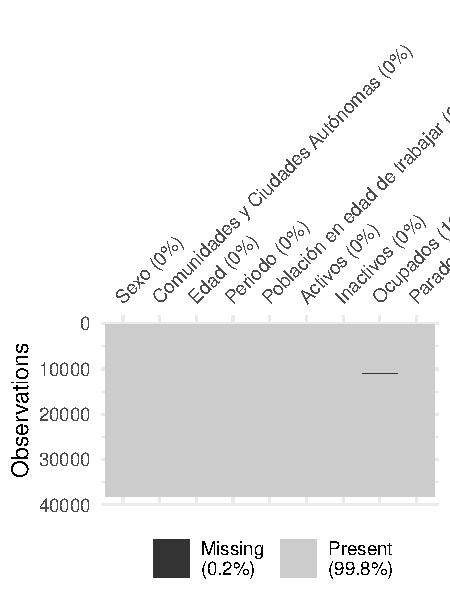
\includegraphics{ProyectoAED2024_files/figure-latex/unnamed-chunk-7-1.pdf}

Existe únicamente un porcentaje muy bajo de valores faltantes en la
columna ``Parados''. Veamos un ejemplo de estos casos.

\begin{Shaded}
\begin{Highlighting}[]
\NormalTok{miss\_datos\_EPA }\OtherTok{\textless{}{-}}\NormalTok{ datos\_EPA }\SpecialCharTok{\%\textgreater{}\%} \FunctionTok{mutate}\NormalTok{(}\AttributeTok{miss\_parados =} \FunctionTok{is.na}\NormalTok{(Parados)) }\SpecialCharTok{\%\textgreater{}\%} \FunctionTok{filter}\NormalTok{(miss\_parados }\SpecialCharTok{==} \ConstantTok{TRUE}\NormalTok{)}
\FunctionTok{lapply}\NormalTok{(miss\_datos\_EPA[,}\FunctionTok{c}\NormalTok{(}\StringTok{"Comunidades y Ciudades Autónomas"}\NormalTok{, }\StringTok{"Edad"}\NormalTok{)], table)}
\end{Highlighting}
\end{Shaded}

\begin{verbatim}
## $`Comunidades y Ciudades Autónomas`
## 
##                      02 Aragón     03 Asturias, Principado de 
##                              1                              3 
##                   06 Cantabria 15 Navarra, Comunidad Foral de 
##                             11                             11 
##                  16 País Vasco                   17 Rioja, La 
##                              2                             14 
##                       18 Ceuta                     19 Melilla 
##                             79                            151 
## 
## $Edad
## 
##   55 y más años De 16 a 19 años De 20 a 24 años De 25 a 34 años De 35 a 44 años 
##             101             114              15               1              13 
## De 45 a 54 años           Total 
##              27               1
\end{verbatim}

Los datos se concentran en Comunidades y Ciudades Autónomas con
proporcionalmente poca población y en rangos de edades donde es poco
habitual estar parado (ya que para que se cumpla dicha condición se debe
estar buscando activamente trabajo). De hecho, el único valor que podría
resultar extraño es que exista un valor faltante para un Total de
edades, pero al comprobar la localización y fecha notamos que es
razonable.

\begin{Shaded}
\begin{Highlighting}[]
\NormalTok{miss\_datos\_EPA[miss\_datos\_EPA}\SpecialCharTok{$}\NormalTok{Edad }\SpecialCharTok{==} \StringTok{"Total"}\NormalTok{,}\FunctionTok{c}\NormalTok{(}\StringTok{"Sexo"}\NormalTok{, }\StringTok{"Comunidades y Ciudades Autónomas"}\NormalTok{, }\StringTok{"Periodo"}\NormalTok{)]}
\end{Highlighting}
\end{Shaded}

\begin{verbatim}
## # A tibble: 1 x 3
##   Sexo    `Comunidades y Ciudades Autónomas` Periodo   
##   <chr>   <chr>                              <date>    
## 1 Hombres 19 Melilla                         2002-06-01
\end{verbatim}

\begin{Shaded}
\begin{Highlighting}[]
\FunctionTok{rm}\NormalTok{(}\AttributeTok{list=}\FunctionTok{c}\NormalTok{(}\StringTok{"miss\_datos\_EPA"}\NormalTok{))}
\end{Highlighting}
\end{Shaded}

Dicho patrón parece reflejar que muy poca población de esas
características se encontraba parada; por tanto, sustituiremos los
valores faltantes del dataset por ceros.

\begin{Shaded}
\begin{Highlighting}[]
\NormalTok{datos\_EPA }\OtherTok{\textless{}{-}}\NormalTok{ datos\_EPA }\SpecialCharTok{\%\textgreater{}\%} \FunctionTok{mutate}\NormalTok{(}\AttributeTok{Parados =} \FunctionTok{ifelse}\NormalTok{(}\FunctionTok{is.na}\NormalTok{(Parados), }\DecValTok{0}\NormalTok{, Parados))}
\end{Highlighting}
\end{Shaded}

\subsection{Clasificación Nacional de Actividades Económicas
(CNAE-2009)}\label{clasificaciuxf3n-nacional-de-actividades-econuxf3micas-cnae-2009}

Este dataset divide los datos según rama de actividad, sexo y fecha en
el periodo comprendido entre el primer trimestre de 2008 y el tercer
trimestre de 2024, usando las mismas unidades que en el resto de
datasets. No obstante, en este caso podemos encontrar los datos
segmentado en dos subconjuntos principales:

· Porcentajes (``Total\_abs''): Representan la proporción de ocupación
de cada rama de actividad con respecto al total del sexo
correspondiente. · Valores absolutos (``Total\_porc''): Proporcionan el
número total de empleados en cada rama.

Esta separación permite analizar tanto las tendencias globales (valores
absolutos) como la estructura relativa de los sectores (porcentajes).

\begin{Shaded}
\begin{Highlighting}[]
\NormalTok{datos\_CNAE }\OtherTok{\textless{}{-}} \FunctionTok{read.csv}\NormalTok{(}\StringTok{"data/CNAE.csv"}\NormalTok{, }\AttributeTok{sep=}\StringTok{";"}\NormalTok{, }\AttributeTok{dec=}\StringTok{","}\NormalTok{)}
\end{Highlighting}
\end{Shaded}

Esta vez al usar la función ``read.csv'' tendremos que modificar el tipo
de dato de la columna ``Total'' de cadena de texto a numérico. Además,
nos encontramos de nuevo con el problema del formato de las fechas, por
lo que volveremos a aplicar la función SacarFechas.

\begin{Shaded}
\begin{Highlighting}[]
\NormalTok{datos\_CNAE}\SpecialCharTok{$}\NormalTok{Total }\OtherTok{\textless{}{-}} \FunctionTok{as.numeric}\NormalTok{(}\FunctionTok{gsub}\NormalTok{(}\StringTok{","}\NormalTok{, }\StringTok{"."}\NormalTok{, }\FunctionTok{gsub}\NormalTok{(}\StringTok{"}\SpecialCharTok{\textbackslash{}\textbackslash{}}\StringTok{."}\NormalTok{, }\StringTok{""}\NormalTok{, datos\_CNAE}\SpecialCharTok{$}\NormalTok{Total)))}
\NormalTok{datos\_CNAE}\SpecialCharTok{$}\NormalTok{Periodo }\OtherTok{\textless{}{-}} \FunctionTok{as.Date}\NormalTok{(}\FunctionTok{sapply}\NormalTok{(datos\_CNAE}\SpecialCharTok{$}\NormalTok{Periodo, sacarFechas), }\AttributeTok{format =} \StringTok{"\%Y{-}\%m{-}\%d"}\NormalTok{)}
\end{Highlighting}
\end{Shaded}

Para diferenciar entre cada tipo de dato (valor absoluto y porcentaje)
vamos a extraerlos en dos datasets para posteriormente realizar un join,
esencialmente como si se realizara un pivote.

\begin{Shaded}
\begin{Highlighting}[]
\NormalTok{datos\_CNAE\_porc }\OtherTok{\textless{}{-}}\NormalTok{ datos\_CNAE[datos\_CNAE}\SpecialCharTok{$}\NormalTok{Unidad}\SpecialCharTok{==}\StringTok{"Porcentaje"}\NormalTok{,]}
\NormalTok{datos\_CNAE\_porc }\OtherTok{\textless{}{-}}\NormalTok{ datos\_CNAE\_porc[, }\SpecialCharTok{!}\FunctionTok{names}\NormalTok{(datos\_CNAE\_porc) }\SpecialCharTok{\%in\%} \StringTok{"Unidad"}\NormalTok{]}

\NormalTok{datos\_CNAE\_abs }\OtherTok{\textless{}{-}}\NormalTok{ datos\_CNAE[datos\_CNAE}\SpecialCharTok{$}\NormalTok{Unidad}\SpecialCharTok{==}\StringTok{"Valor absoluto"}\NormalTok{,]}
\NormalTok{datos\_CNAE\_abs }\OtherTok{\textless{}{-}}\NormalTok{ datos\_CNAE\_abs[, }\SpecialCharTok{!}\FunctionTok{names}\NormalTok{(datos\_CNAE\_abs) }\SpecialCharTok{\%in\%} \StringTok{"Unidad"}\NormalTok{]}

\ControlFlowTok{if}\NormalTok{ (}\FunctionTok{dim}\NormalTok{(datos\_CNAE\_abs)[}\DecValTok{1}\NormalTok{] }\SpecialCharTok{==} \FunctionTok{dim}\NormalTok{(datos\_CNAE\_porc)[}\DecValTok{1}\NormalTok{] }\SpecialCharTok{\&} \FunctionTok{dim}\NormalTok{(datos\_CNAE\_abs)[}\DecValTok{2}\NormalTok{] }\SpecialCharTok{==} \FunctionTok{dim}\NormalTok{(datos\_CNAE\_porc)[}\DecValTok{2}\NormalTok{])\{}
\NormalTok{  datos\_CNAE }\OtherTok{\textless{}{-}} \FunctionTok{left\_join}\NormalTok{(datos\_CNAE\_abs, datos\_CNAE\_porc, }\AttributeTok{by =} \FunctionTok{c}\NormalTok{(}\StringTok{"Rama.de.actividad.CNAE.2009"}\NormalTok{, }\StringTok{"Sexo"}\NormalTok{, }\StringTok{"Periodo"}\NormalTok{), }\AttributeTok{suffix =} \FunctionTok{c}\NormalTok{(}\StringTok{"\_abs"}\NormalTok{, }\StringTok{"\_porc"}\NormalTok{))}
\NormalTok{\}}

\FunctionTok{rm}\NormalTok{(}\AttributeTok{list =} \FunctionTok{c}\NormalTok{(}\StringTok{"datos\_CNAE\_abs"}\NormalTok{, }\StringTok{"datos\_CNAE\_porc"}\NormalTok{))}
\end{Highlighting}
\end{Shaded}

Una vez tenemos la tabla unificada es recomendable realizar un análisis
de datos faltantes.

\begin{Shaded}
\begin{Highlighting}[]
\FunctionTok{vis\_miss}\NormalTok{(datos\_CNAE)}
\end{Highlighting}
\end{Shaded}

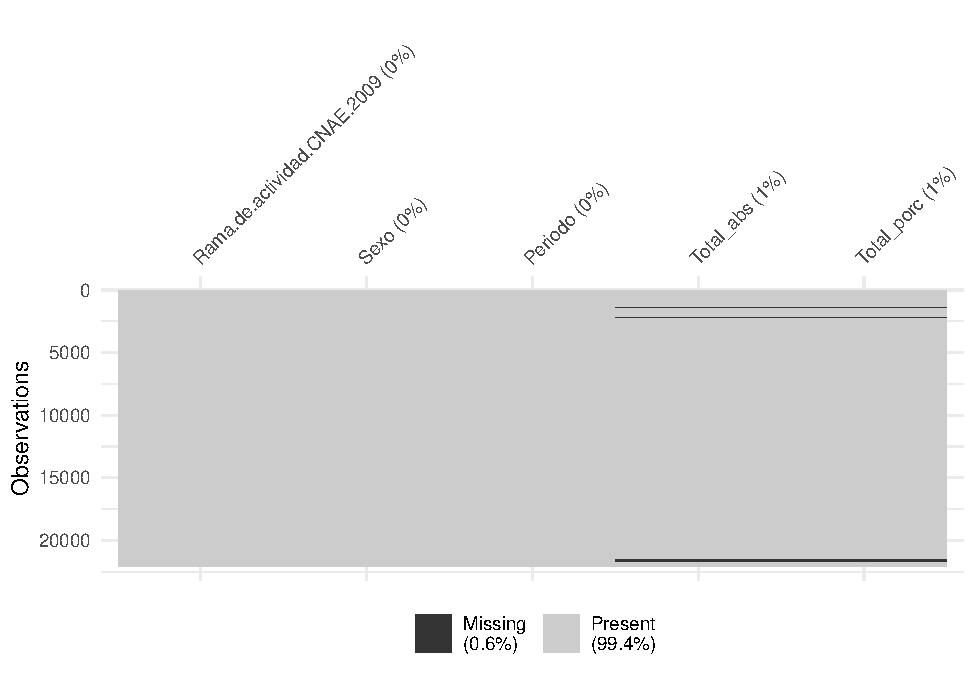
\includegraphics{ProyectoAED2024_files/figure-latex/unnamed-chunk-14-1.pdf}

Observamos que para un pequeño subconjunto de filas no existen cifras
totales. Veamos si siguen algún patrón.

\begin{Shaded}
\begin{Highlighting}[]
\NormalTok{miss\_datos\_CNAE }\OtherTok{\textless{}{-}}\NormalTok{ datos\_CNAE }\SpecialCharTok{\%\textgreater{}\%} \FunctionTok{mutate}\NormalTok{(}\AttributeTok{miss\_total =} \FunctionTok{is.na}\NormalTok{(Total\_abs)) }\SpecialCharTok{\%\textgreater{}\%} \FunctionTok{filter}\NormalTok{(miss\_total }\SpecialCharTok{==} \ConstantTok{TRUE}\NormalTok{)}
\FunctionTok{head}\NormalTok{(}\FunctionTok{unique}\NormalTok{(miss\_datos\_CNAE}\SpecialCharTok{$}\NormalTok{Rama.de.actividad.CNAE}\FloatTok{.2009}\NormalTok{), }\DecValTok{4}\NormalTok{)}
\end{Highlighting}
\end{Shaded}

\begin{verbatim}
## [1] "05 Extracción de antracita, hulla y lignito"         
## [2] "06 Extracción de crudo de petróleo y gas natural"    
## [3] "07 Extracción de minerales metálicos"                
## [4] "09 Actividades de apoyo a las industrias extractivas"
\end{verbatim}

\begin{Shaded}
\begin{Highlighting}[]
\FunctionTok{rm}\NormalTok{(}\AttributeTok{list=}\FunctionTok{c}\NormalTok{(}\StringTok{"miss\_datos\_CNAE"}\NormalTok{))}
\end{Highlighting}
\end{Shaded}

Notamos que los valores faltantes se encuentran en ramas de actividades
poco comunes relacionadas con la industria pesada, por lo que dichos NA
reflejarán que muy poca población se dedica a ello, probablemente menos
del mínimo registrable; en consecuencia sustituiremos dichos valores por
ceros.

\begin{Shaded}
\begin{Highlighting}[]
\NormalTok{datos\_CNAE }\OtherTok{\textless{}{-}}\NormalTok{ datos\_CNAE }\SpecialCharTok{\%\textgreater{}\%} \FunctionTok{mutate}\NormalTok{(}\AttributeTok{Total\_abs =} \FunctionTok{ifelse}\NormalTok{(}\FunctionTok{is.na}\NormalTok{(Total\_abs), }\DecValTok{0}\NormalTok{, Total\_abs)) }\SpecialCharTok{\%\textgreater{}\%} \FunctionTok{mutate}\NormalTok{(}\AttributeTok{Total\_porc =} \FunctionTok{ifelse}\NormalTok{(}\FunctionTok{is.na}\NormalTok{(Total\_porc), }\DecValTok{0}\NormalTok{, Total\_porc))}
\end{Highlighting}
\end{Shaded}

Por último, añadiremos una columna que calcula la variación entre un
periodo y el siguiente, lo que permitirá identificar momentos de cambio
significativo en el mercado laboral, detectando tendencias positivas o
negativas a lo largo del tiempo. Esto también permitirá ver de manera
rápida la estacionalidad de la ocupación, sobre todo en ciertas ramas de
actividad.

Es importante menciona que realizar las diferencias entre un periodo y
el siguiente genera NAs para el primer periodo de cada rama, por lo que
sustituiremos estos valores faltantes por ceros.

\begin{Shaded}
\begin{Highlighting}[]
\NormalTok{datos\_CNAE}\SpecialCharTok{$}\NormalTok{Diferencia\_Total }\OtherTok{\textless{}{-}} \ConstantTok{NA}

\ControlFlowTok{for}\NormalTok{ (sexo }\ControlFlowTok{in} \FunctionTok{unique}\NormalTok{(datos\_CNAE}\SpecialCharTok{$}\NormalTok{Sexo)) \{}
  \ControlFlowTok{for}\NormalTok{ (rama }\ControlFlowTok{in} \FunctionTok{unique}\NormalTok{(datos\_CNAE}\SpecialCharTok{$}\NormalTok{Rama.de.actividad.CNAE}\FloatTok{.2009}\NormalTok{)) \{}
\NormalTok{    subset }\OtherTok{\textless{}{-}}\NormalTok{ datos\_CNAE[datos\_CNAE}\SpecialCharTok{$}\NormalTok{Sexo }\SpecialCharTok{==}\NormalTok{ sexo }\SpecialCharTok{\&} 
\NormalTok{                        datos\_CNAE}\SpecialCharTok{$}\NormalTok{Rama.de.actividad.CNAE}\FloatTok{.2009} \SpecialCharTok{==}\NormalTok{ rama, ]}
    
\NormalTok{    datos\_CNAE}\SpecialCharTok{$}\NormalTok{Diferencia\_Total[datos\_CNAE}\SpecialCharTok{$}\NormalTok{Sexo }\SpecialCharTok{==}\NormalTok{ sexo }\SpecialCharTok{\&} 
\NormalTok{                                datos\_CNAE}\SpecialCharTok{$}\NormalTok{Rama.de.actividad.CNAE}\FloatTok{.2009} \SpecialCharTok{==}\NormalTok{ rama }\SpecialCharTok{\&}\NormalTok{ datos\_CNAE}\SpecialCharTok{$}\NormalTok{Periodo }\SpecialCharTok{!=} \FunctionTok{min}\NormalTok{(datos\_CNAE}\SpecialCharTok{$}\NormalTok{Periodo)] }\OtherTok{\textless{}{-}} 
      \FunctionTok{diff}\NormalTok{(subset}\SpecialCharTok{$}\NormalTok{Total\_abs)}
\NormalTok{  \}}
\NormalTok{\}}

\NormalTok{datos\_CNAE}\SpecialCharTok{$}\NormalTok{Diferencia\_Total[datos\_CNAE}\SpecialCharTok{$}\NormalTok{Periodo }\SpecialCharTok{==} \FunctionTok{min}\NormalTok{(datos\_CNAE}\SpecialCharTok{$}\NormalTok{Periodo)] }\OtherTok{\textless{}{-}} \DecValTok{0}
\FunctionTok{rm}\NormalTok{(}\AttributeTok{list =} \FunctionTok{c}\NormalTok{(}\StringTok{"subset"}\NormalTok{))}
\end{Highlighting}
\end{Shaded}


%%%%%%%%%%%%%%%%%%%%%%%%%%%%%%%%%%%%%%%%%%

\vspace{6pt}

%%%%%%%%%%%%%%%%%%%%%%%%%%%%%%%%%%%%%%%%%%
%% optional

% Only for the journal Methods and Protocols:
% If you wish to submit a video article, please do so with any other supplementary material.
% \supplementary{The following supporting information can be downloaded at: \linksupplementary{s1}, Figure S1: title; Table S1: title; Video S1: title. A supporting video article is available at doi: link.}

%%%%%%%%%%%%%%%%%%%%%%%%%%%%%%%%%%%%%%%%%%







%%%%%%%%%%%%%%%%%%%%%%%%%%%%%%%%%%%%%%%%%%
%% Optional

%% Only for journal Encyclopedia


%%%%%%%%%%%%%%%%%%%%%%%%%%%%%%%%%%%%%%%%%%
%% Optional
\input{"appendix.tex"}
%%%%%%%%%%%%%%%%%%%%%%%%%%%%%%%%%%%%%%%%%%
\begin{adjustwidth}{-\extralength}{0cm}

%\printendnotes[custom] % Un-comment to print a list of endnotes


\reftitle{References}
\bibliography{mybibfile.bib}

% If authors have biography, please use the format below
%\section*{Short Biography of Authors}
%\bio
%{\raisebox{-0.35cm}{\includegraphics[width=3.5cm,height=5.3cm,clip,keepaspectratio]{Definitions/author1.pdf}}}
%{\textbf{Firstname Lastname} Biography of first author}
%
%\bio
%{\raisebox{-0.35cm}{\includegraphics[width=3.5cm,height=5.3cm,clip,keepaspectratio]{Definitions/author2.jpg}}}
%{\textbf{Firstname Lastname} Biography of second author}

%%%%%%%%%%%%%%%%%%%%%%%%%%%%%%%%%%%%%%%%%%
%% for journal Sci
%\reviewreports{\\
%Reviewer 1 comments and authors’ response\\
%Reviewer 2 comments and authors’ response\\
%Reviewer 3 comments and authors’ response
%}
%%%%%%%%%%%%%%%%%%%%%%%%%%%%%%%%%%%%%%%%%%
\PublishersNote{}
\end{adjustwidth}


\end{document}
